\documentclass[preview]{standalone}
\usepackage[margin=0.5in]{geometry} % Adjusts the margins and sets landscape mode
\usepackage{graphicx} % Required for inserting images

\usepackage{amsmath,amssymb,amsthm}
\usepackage{tikz}

\begin{document}

\begin{center}
\begin{tikzpicture}
    % helpful origin marker
    % \node at (0,0) {O};

    \draw[line width = 2pt] (3, -4) circle (0.75);
    \node at (3, -4) {\Large $\textbf{\text{x}}_T$};

    \node at (3, -2.9) {\large $\mathcal{N}(0,\,\textbf{\text{I}})$};

    \begin{scope}[local bounding box=image box]
        \node at (3, -8.5) {
\includegraphics[width = 2.5cm]{xTimagediffv2.jpg}};
    \end{scope}
    % Now draw the border around the specific local bounding box
    \draw [white, rounded corners=0.5cm, line width=0.2cm] 
    (image box.north west) -- 
    (image box.north east) --
    (image box.south east) --
    (image box.south west) -- cycle
    ;

    % \draw[ultra thick, ->] (4, -4) -- (6,-4);

    % Horz Ellipsis
    \draw[fill = black, ultra thick] (4.5, -4) circle (0.05);
    \draw[fill = black, ultra thick] (5, -4) circle (0.05);
    \draw[fill = black, ultra thick] (5.5, -4) circle (0.05);

    \draw[line width = 2pt] (7, -4) circle (0.75);
    \node at (7, -4) {\Large $\textbf{\text{x}}_{t}$};

    \begin{scope}[local bounding box=image box]
        \node at (7, -8.5) {
\includegraphics[width = 2.5cm]{xlatertimagediffv2.jpg}};
    \end{scope}
    % Now draw the border around the specific local bounding box
    \draw [white, rounded corners=0.5cm, line width=0.2cm] 
    (image box.north west) -- 
    (image box.north east) --
    (image box.south east) --
    (image box.south west) -- cycle
    ;



    \draw[ultra thick, ->] (8,-4) -- (10,-4);
    \node at (9, -4.5) {\Large $p_{\theta}(\textbf{\text{x}}_{t-1} | \textbf{\text{x}}_{t})$};

    
    
    \draw[line width = 2pt] (11, -4) circle (0.75);
    \node at (11, -4) {\Large $\textbf{\text{x}}_{t-1}$};
    
    \begin{scope}[local bounding box=image box]
        \node at (11, -8.5) {
\includegraphics[width = 2.5cm]{xinttimagediffv2.jpg}};
    \end{scope}
    % Now draw the border around the specific local bounding box
    \draw [white, rounded corners=0.5cm, line width=0.2cm] 
    (image box.north west) -- 
    (image box.north east) --
    (image box.south east) --
    (image box.south west) -- cycle
    ;
    

    % Horz Ellipsis
    \draw[fill = black, ultra thick] (12.5, -4) circle (0.05);
    \draw[fill = black, ultra thick] (13, -4) circle (0.05);
    \draw[fill = black, ultra thick] (13.5, -4) circle (0.05);

    \draw[line width = 2pt] (15, -4) circle (0.75);
    \node at (15, -4) {\Large $\textbf{\text{x}}_{0}$};
    \begin{scope}[local bounding box=image box]
        \node at (15, -8.5) {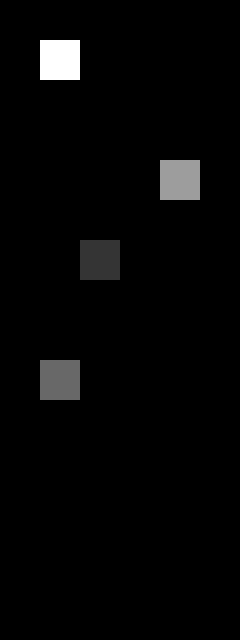
\includegraphics[width = 2.5cm]{x0imagediffv2.jpg}};
    \end{scope}
    % Now draw the border around the specific local bounding box
    \draw [white, rounded corners=0.5cm, line width=0.2cm] 
    (image box.north west) -- 
    (image box.north east) --
    (image box.south east) --
    (image box.south west) -- cycle
    ;
    
    
    % Curved line from x_0 to x_t
    \draw[ultra thick, dash pattern=on 5pt off 4.5pt, ->] (15, -3) to [out=160,in=20] (7, -3);
    \node at (11,-1.75) {\Large $q(\textbf{\text{x}}_t | \textbf{\text{x}}_{0})$};

    \draw[ultra thick, ->] (16, -4) -- (17,-4);
    % Specify that "NOTE: Hg ... is a compound found in SuperCon, not generated by SuperDiff, that is used for visualization purposes only (also stuff about how images are for visualization only and are created by SuperDiff noising, not actual SuperDiff denoising outputs).

    % Y1Ba2Cu3O4.86
    \node at (18.6, -4) {\Large $\mathrm{YBa_{2}Cu_{3}O_{4.86}}$};
    
    
\end{tikzpicture}
\end{center}


\end{document}
